\documentclass[12pt, a4paper]{report}

% ==== Paket dasar ====
\usepackage[utf8]{inputenc}
\usepackage[T1]{fontenc}
\usepackage[indonesian]{babel}
\usepackage{times}

% ==== Layout halaman ====
\usepackage[top=4cm, left=4cm, bottom=3cm, right=3cm,
headheight=15pt]{geometry}
\usepackage{setspace}
\onehalfspacing
% Indentasi alinea 6 ketukan (panduan: 0,5 inci = 1,27 cm)
\setlength{\parindent}{1.27cm}
% Nomor halaman arab di kanan atas; halaman awal bab tetap tengah bawah
\usepackage{fancyhdr}
\fancyhf{}
\fancyhead[R]{\thepage}
\renewcommand{\headrulewidth}{0pt}

% ==== Gambar, tabel, dan lainnya ====
\usepackage{graphicx}
\graphicspath{{gambar/}}
\usepackage{booktabs}
\usepackage{caption}
% Judul tabel/gambar font 11, dua ketukan setelah nomor, baris lanjutan menggantung
\captionsetup{font=small, labelsep=quad, format=hang}
% Nomor tabel angka arab per bab (Tabel 2.1); nomor gambar berurutan global
\renewcommand{\thetable}{\arabic{chapter}.\arabic{table}}
\counterwithout{figure}{chapter}
\usepackage{amsmath}
\usepackage{amssymb}
\usepackage{tikz}
\usetikzlibrary{arrows.meta, positioning}
\usepackage{hyperref}
\hypersetup{hidelinks}

% ==== Daftar pustaka ====
\usepackage{csquotes}
\usepackage[backend=biber, style=authoryear, maxcitenames=2,
  maxbibnames=99, dashed=false, uniquename=false,
uniquelist=false]{biblatex}
% Lokalisasi Indonesia disediakan lewat indonesian.lbx di folder proyek
% Format sitasi (Penulis, Tahun) seperti APA
\renewcommand*{\nameyeardelim}{\addcomma\space}
% Daftar pustaka spasi 1 dengan jarak antarentri 6 pt
\setlength{\bibitemsep}{6pt}
\addbibresource{daftar-pustaka.bib}

% ==== Format judul bab ====
\usepackage{titlesec}
\usepackage{titletoc}
\renewcommand{\thechapter}{\Roman{chapter}}
\renewcommand{\thesection}{\arabic{chapter}.\arabic{section}}
\titleformat{\chapter}[display]
{\centering\bfseries\normalsize}
{BAB \thechapter}{0.5em}{\MakeUppercase}
\titlespacing*{\chapter}{0pt}{0pt}{2em}
\titleformat{\section}{\bfseries\normalsize}{\thesection}{1em}{}
\titleformat{\subsection}{\bfseries\normalsize}{\thesubsection}{1em}{}
\titlespacing*{\section}{0pt}{12pt}{6pt}
\titlespacing*{\subsection}{0pt}{12pt}{6pt}

% ==== Format daftar isi ====
\titlecontents{chapter}[0pt]
{\addvspace{1em}\bfseries}
{BAB \thecontentslabel\ }
{}
{\titlerule*[0.7pc]{.}\contentspage}

% ==== Metadata ====
\newcommand{\judul}{Asisten Akademik Berbasis Kecerdasan Buatan untuk Manajemen Tugas dan Jadwal Kuliah Mahasiswa}
\newcommand{\namapenulis}{Jouska Brillian Putra Purnomo}
\newcommand{\nim}{220113003}
\newcommand{\prodi}{S1 Teknologi Informasi}
\newcommand{\fakultas}{Fakultas Sains dan Teknologi}
\newcommand{\universitas}{Universitas Harapan Bangsa}

\begin{document}

% ==== Halaman judul ====
\begin{titlepage}
  \centering
  {\Large\bfseries PROPOSAL TUGAS AKHIR\\INOVASI/TEKNOLOGI TEPAT GUNA\par}
  \vspace{1.5cm}
  {\Large\bfseries \MakeUppercase{\judul}\par}
  \vspace{2cm}
  
\includegraphics[width=5cm]{uhb-logo}
  \vfill
  {\large Disusun oleh:\par}
  \vspace{0.5cm}
  {\large\bfseries \underline{\MakeUppercase{\namapenulis}}\par}
  {\large NIM \nim\par}
  \vfill
  {\large PROGRAM STUDI TEKNOLOGI INFORMASI\par}
  {\large FAKULTAS SAINS DAN TEKNOLOGI\par}
  {\large UNIVERSITAS HARAPAN BANGSA\par}
  {\large \the\year\par}
\end{titlepage}


% ==== Halaman awal (nomor romawi) ====
\pagenumbering{roman}
\chapter*{Halaman Pengesahan}
\addcontentsline{toc}{chapter}{HALAMAN PENGESAHAN}

\begin{center}
  {\bfseries HALAMAN PENGESAHAN\\PROPOSAL TUGAS AKHIR INOVASI/TEKNOLOGI TEPAT GUNA}
\end{center}

\vspace{1em}
\noindent
\begin{tabular}{@{}p{5cm}@{ : }p{9cm}@{}}
  Judul Tugas Akhir & \judul \\
  Nama Mahasiswa    & \namapenulis \\
  NIM               & \nim \\
  Program Studi     & \prodi \\
  Fakultas          & \fakultas \\
\end{tabular}

\vfill

\begin{center}
  Purwokerto, \today
\end{center}

\vspace{1em}
\noindent
\begin{tabular}{@{}p{7cm}p{7cm}@{}}
  \centering Menyetujui,\\Dosen Pembimbing & \centering Mahasiswa \tabularnewline
  \vspace{2.5cm} & \vspace{2.5cm} \tabularnewline
  \centering\underline{Anggit Wirasto, S.Si., M.Eng.
  }\\NIDN. 0625068201 & \centering\underline{\namapenulis}\\NIM. \nim \tabularnewline
\end{tabular}

\vspace{2em}
\begin{center}
  Mengetahui,\\Ketua Program Studi \prodi

  \vspace{2.5cm}
  \underline{Dr. Imam Ahmad Ashari, S.Kom., M.Kom.
  }\\NIDN. 0623089401
\end{center}
\clearpage

\tableofcontents
\clearpage
\phantomsection
\addcontentsline{toc}{chapter}{DAFTAR GAMBAR}
\listoffigures
\clearpage
\phantomsection
\addcontentsline{toc}{chapter}{DAFTAR TABEL}
\listoftables
\clearpage
\chapter*{Ringkasan Proposal}
\addcontentsline{toc}{chapter}{RINGKASAN PROPOSAL}

% Ringkasan maksimum satu halaman, ditulis dengan jarak satu spasi.
\begin{singlespace}
  Mahasiswa kerap kesulitan mengelola tugas, jadwal kuliah, dan informasi
  akademik yang tersebar di berbagai kanal seperti email kampus, grup pesan,
  sistem pembelajaran daring, dan pengumuman dosen. Ketidakteraturan ini
  berdampak pada terlewatnya tenggat, keterlambatan pengumpulan tugas,
  meningkatnya prokrastinasi akademik, dan menurunnya kualitas belajar.
  Aplikasi manajemen tugas yang umum digunakan masih menuntut pengguna
  memasukkan seluruh data secara manual, padahal sumber informasi tugas
  terbesar mahasiswa justru berada di email kampus yang tidak terstruktur.
  Proposal ini mengusulkan pengembangan \textbf{Welya}, sebuah produk
  digital berupa asisten akademik berbasis kecerdasan buatan (AI) yang
  membantu mahasiswa mengelola tugas, jadwal, email kampus, dan kerja
  kelompok dalam satu tempat.

  Welya terintegrasi dengan Gmail, Google Tasks, dan Google Calendar melalui
  API resmi dengan otorisasi OAuth 2.0. Sistem memanfaatkan model bahasa
  besar (\emph{large language model}/LLM) untuk menganalisis email kampus
  secara otomatis, mendeteksi email yang mengandung penugasan, mengekstraksi
  atribut tugas seperti judul, mata kuliah, dan tenggat, lalu memecah tugas
  menjadi subtask beserta estimasi waktu pengerjaannya. Seluruh tenggat dan
  jadwal kuliah disajikan dalam satu dasbor dengan prioritas harian,
  dilengkapi kalender tersinkron, pencarian cerdas atas tugas, materi, dan
  catatan, serta ruang kerja kolaborasi untuk kerja kelompok. Kebaruan
  produk ini terletak pada deteksi tugas otomatis dari email kampus
  berbahasa Indonesia --- kemampuan yang belum tersedia pada aplikasi
  manajemen tugas populer seperti Google Tasks, Todoist, maupun Notion.

  Pengembangan dilakukan secara iteratif dengan metode \emph{prototype}
  melalui tahapan analisis kebutuhan, perancangan sistem, implementasi,
  pengujian, dan evaluasi kepada pengguna. Produk dibangun sebagai aplikasi
  web sekaligus aplikasi desktop sehingga dapat diakses lintas perangkat.
  Evaluasi mencakup pengujian fungsional \emph{black-box}, pengukuran
  ketepatan deteksi tugas dengan \emph{precision} dan \emph{recall}
  bertarget minimal 80\%, serta kuesioner \emph{System Usability Scale}
  (SUS) kepada minimal 10 responden mahasiswa dengan target skor di atas 68.

  Target luaran tugas akhir ini berupa aplikasi Welya (web dan desktop)
  yang berfungsi penuh dan siap diuji coba, laporan tugas akhir, artikel
  publikasi ilmiah, serta pendaftaran Hak Kekayaan Intelektual (HKI).
  Kehadiran Welya diharapkan membantu mahasiswa mengelola aktivitas
  akademiknya secara lebih teratur sekaligus menjadi contoh penerapan
  teknologi AI dalam mendukung produktivitas akademik di lingkungan
  perguruan tinggi.

  \vspace{0.5em}
  \noindent\textbf{Kata kunci}: asisten akademik, kecerdasan buatan,
  manajemen tugas, model bahasa besar, integrasi Google.
\end{singlespace}
\clearpage


% ==== Isi (nomor arab) ====
\pagenumbering{arabic}
\pagestyle{fancy}
\chapter{PENDAHULUAN}

\section{Latar Belakang}
Kehidupan akademik mahasiswa menuntut pengelolaan banyak hal sekaligus:
tugas kuliah dengan tenggat yang berbeda-beda, jadwal perkuliahan, email
dari dosen dan kampus, serta koordinasi kerja kelompok. Informasi tersebut
tersebar di berbagai kanal --- email kampus, grup pesan instan, sistem
pembelajaran daring, dan pengumuman lisan di kelas --- sehingga mahasiswa
sering melewatkan tenggat atau kesulitan menentukan prioritas pengerjaan.

Kemampuan manajemen waktu terbukti berpengaruh positif terhadap prestasi
akademik mahasiswa \parencite{kamilatunnisa2025}. Sebaliknya, kegagalan
regulasi diri seperti prokrastinasi akademik berhubungan erat dengan
menurunnya kinerja dan kesejahteraan mahasiswa \parencite{fadila2024}.
Sayangnya, aplikasi manajemen
tugas yang umum digunakan (daftar tugas dan kalender generik) masih
menuntut pengguna memasukkan seluruh data secara manual, padahal sumber
informasi tugas terbesar mahasiswa justru berada di email kampus dan
dokumen perkuliahan yang tidak terstruktur.

Perkembangan kecerdasan buatan, khususnya model bahasa besar
(\emph{large language model}/LLM), membuka peluang untuk mengotomatiskan
pengelolaan informasi akademik dan terbukti bermanfaat sebagai asisten
pembelajaran digital bagi mahasiswa
\parencite{johan2026, hidayah2025}. Email kampus dapat dianalisis untuk mendeteksi tugas
secara otomatis, tugas dapat dipecah menjadi subtask dengan estimasi waktu,
dan seluruh tenggat dapat disajikan dalam satu dasbor terpadu.

Berdasarkan permasalahan tersebut, tugas akhir ini mengusulkan pengembangan
\textbf{Welya}, asisten akademik berbasis AI dalam bentuk produk digital
(aplikasi web dan desktop) yang membantu mahasiswa mengelola tugas, jadwal, email
kampus, dan kerja kelompok dalam satu tempat. Welya terintegrasi dengan
Gmail, Google Tasks, dan Google Calendar sehingga tugas terdeteksi
otomatis, tersusun rapi, dan mudah dipantau melalui satu dasbor.

\section{Rumusan Masalah}
\begin{enumerate}
  \item Bagaimana merancang dan membangun asisten akademik berbasis AI
    yang mampu mendeteksi tugas secara otomatis dari email kampus?
  \item Bagaimana mengintegrasikan aplikasi dengan layanan Gmail, Google
    Tasks, dan Google Calendar agar tugas dan jadwal mahasiswa
    terkelola dalam satu dasbor?
  \item Bagaimana tingkat kebermanfaatan dan kemudahan penggunaan
    aplikasi bagi mahasiswa?
\end{enumerate}

\section{Tujuan}
\begin{enumerate}
  \item Menghasilkan produk digital Welya berupa aplikasi web dan desktop asisten
    akademik berbasis AI yang siap diuji coba.
  \item Mengimplementasikan integrasi Gmail, Google Tasks, dan Google
    Calendar untuk deteksi tugas dan sinkronisasi jadwal otomatis.
  \item Mengukur kebermanfaatan dan kemudahan penggunaan aplikasi melalui
    uji coba kepada mahasiswa.
\end{enumerate}

\section{Manfaat}
\begin{enumerate}
  \item Bagi mahasiswa: membantu mengatur tugas, jadwal, dan email kampus
    sehingga kuliah lebih teratur dan tenggat tidak terlewat.
  \item Bagi institusi: menjadi contoh penerapan teknologi AI dalam
    mendukung produktivitas akademik mahasiswa.
  \item Bagi penulis: menerapkan ilmu rekayasa perangkat lunak dan
    kecerdasan buatan dalam produk nyata yang berpotensi memperoleh
    HKI.
\end{enumerate}

\section{Batasan Masalah}
\begin{enumerate}
  \item Aplikasi tersedia sebagai aplikasi web dan aplikasi desktop
    serta menargetkan pengguna mahasiswa.
  \item Integrasi layanan pihak ketiga terbatas pada Gmail, Google Tasks,
    dan Google Calendar.
  \item Deteksi tugas otomatis berfokus pada email kampus berbahasa
    Indonesia.
  \item Uji coba dilakukan pada lingkup terbatas mahasiswa sebagai
    pengguna awal.
\end{enumerate}

\chapter{KAJIAN PUSTAKA}

\section{Manajemen Tugas dan Waktu Akademik}
Manajemen waktu adalah proses merencanakan dan mengendalikan penggunaan
waktu untuk mencapai tujuan tertentu. Dalam konteks akademik, perilaku
manajemen waktu meliputi penetapan tujuan dan prioritas, mekanisme
perencanaan (membuat daftar tugas dan jadwal), serta preferensi terhadap
keteraturan. Penelitian pada mahasiswa di Indonesia menunjukkan bahwa
perilaku manajemen waktu berpengaruh positif dan signifikan terhadap
prestasi akademik mahasiswa \parencite{kamilatunnisa2025}.

Di sisi lain, prokrastinasi akademik --- menunda pekerjaan meskipun sadar
akan konsekuensinya --- merupakan kegagalan regulasi diri yang umum
terjadi pada mahasiswa; semakin rendah regulasi diri mahasiswa, semakin
tinggi kecenderungan prokrastinasi akademiknya \parencite{fadila2024}. Salah
satu pemicunya adalah beban kognitif dalam
mengingat dan mengorganisasi banyak tugas dari berbagai sumber. Sistem
yang mampu mengumpulkan, memecah, dan menjadwalkan tugas secara otomatis
berpotensi menurunkan beban tersebut dan mendorong perilaku belajar yang
lebih teratur.

\section{Kecerdasan Buatan dan Model Bahasa Besar}
Kecerdasan buatan (\emph{artificial intelligence}) adalah bidang ilmu yang
mempelajari sistem cerdas yang mampu memahami lingkungannya dan mengambil
tindakan untuk mencapai tujuan tertentu. Salah satu inovasinya yang
berkembang paling pesat adalah model bahasa besar (\emph{large language
model}/LLM), yaitu model bahasa berbasis AI yang mampu memahami dan
menghasilkan teks dalam bahasa alami \parencite{johan2026}.

Kajian terhadap pemanfaatan LLM di perguruan tinggi menunjukkan bahwa LLM
dapat membantu mahasiswa memahami materi perkuliahan, memperoleh
informasi dengan cepat, mendukung pembelajaran mandiri, serta
meningkatkan interaksi dalam proses belajar apabila digunakan secara
bijak dan didukung literasi digital yang memadai \parencite{johan2026}.
Chatbot berbasis AI juga terbukti berperan sebagai asisten virtual yang
personal, responsif, dan adaptif dalam pembelajaran digital, termasuk
mendukung pengembangan keterampilan manajemen waktu dan kemandirian
belajar \parencite{hidayah2025}.
Dalam Welya, kemampuan ini dimanfaatkan untuk tiga hal: (1) menyaring
email kampus yang mengandung penugasan, (2) mengekstraksi atribut tugas
seperti judul, mata kuliah, dan tenggat, serta (3) memecah tugas menjadi
subtask dengan estimasi waktu pengerjaan.

\section{Aplikasi Web, Aplikasi Desktop, dan Integrasi Layanan Google}
Aplikasi web dipilih karena dapat diakses lintas perangkat tanpa
instalasi, sementara versi desktop dibangun menggunakan kerangka kerja
Tauri yang membungkus antarmuka web yang sama menjadi aplikasi native
yang ringan. Penelitian sejenis menunjukkan bahwa aplikasi manajemen tugas
berbasis web dengan fitur pengingat otomatis, prioritas, dan kalender
interaktif mampu meningkatkan disiplin dan efisiensi pengelolaan waktu
mahasiswa \parencite{panjaitan2025}.

Integrasi dengan ekosistem Google dilakukan melalui API resmi Gmail,
Google Tasks, dan Google Calendar. Pemanfaatan Google Calendar untuk
otomatisasi penjadwalan dan pengingat tenggat terbukti meningkatkan
kepatuhan terhadap tenggat waktu sekaligus mengurangi kesalahan
penjadwalan manual \parencite{setiawan2025}, dan integrasi Google Calendar
API mampu menyinkronkan tugas ke kalender pribadi pengguna secara
\emph{real-time} \parencite{moedjahedy2025}. Otorisasi akses data pengguna
menggunakan protokol OAuth 2.0, standar industri yang memungkinkan
aplikasi pihak ketiga mengakses sumber daya pengguna secara terbatas
tanpa menyimpan kata sandi; penerapannya terbukti meningkatkan keamanan
autentikasi secara signifikan \parencite{arianto2025}. Dengan pendekatan ini,
data
tetap berada di akun Google milik pengguna dan aplikasi hanya meminta
cakupan izin yang diperlukan.

Karena sistem memproses isi email pengguna, aspek privasi menjadi
perhatian utama dalam perancangan. Akses data hanya dilakukan setelah
persetujuan eksplisit pengguna, cakupan izin (\emph{scope}) OAuth
dibatasi seminimal mungkin, data yang disimpan hanya hasil ekstraksi
tugas --- bukan salinan isi email --- dan pengguna dapat mencabut akses
kapan saja. Praktik ini sejalan dengan prinsip pelindungan data pribadi
sebagaimana diatur dalam Undang-Undang Nomor 27 Tahun 2022 tentang
Pelindungan Data Pribadi.

\section{\emph{System Usability Scale} (SUS)}
SUS adalah instrumen baku berisi sepuluh pernyataan berskala Likert untuk
mengukur kebergunaan suatu sistem secara cepat dan andal, dan telah
banyak digunakan dalam evaluasi aplikasi di Indonesia \parencite{dyayu2023}.
Skor akhir berada pada rentang 0--100 dengan nilai 68 sebagai ambang
rata-rata industri. Instrumen ini digunakan pada tahap evaluasi untuk
mengukur kemudahan penggunaan Welya oleh mahasiswa.

\section{Penelitian dan Produk Sejenis}
Beberapa produk manajemen tugas telah tersedia secara luas, di antaranya
Google Tasks, Todoist, dan Notion. Ketiganya andal sebagai pencatat tugas,
tetapi memiliki keterbatasan dalam konteks akademik mahasiswa Indonesia,
sebagaimana diringkas pada Tabel~\ref{tab:perbandingan}.

\begin{table}[htbp]
  \centering
  \caption{Perbandingan Welya dengan produk sejenis}
  \label{tab:perbandingan}
  \small
  \begin{tabular}{@{}p{4.2cm}cccc@{}}
    \toprule
    Fitur & Google Tasks & Todoist & Notion & Welya \\
    \midrule
    Pencatatan tugas manual        & $\checkmark$ & $\checkmark$ & $\checkmark$ & $\checkmark$ \\
    Deteksi tugas dari email       & --           & --           & --           & $\checkmark$ \\
    Subtask + estimasi waktu (AI)  & --           & --           & --           & $\checkmark$ \\
    Kalender jadwal kuliah         & --           & $\checkmark$ & $\checkmark$ & $\checkmark$ \\
    Pencarian cerdas (AI)          & --           & --           & $\checkmark$ & $\checkmark$ \\
    Berfokus konteks akademik      & --           & --           & --           & $\checkmark$ \\
    \bottomrule
  \end{tabular}
\end{table}

Kesenjangan (\emph{gap}) yang mendasari inovasi ini adalah belum adanya
asisten akademik yang mendeteksi tugas secara otomatis dari email kampus
berbahasa Indonesia, memecahnya menjadi subtask beserta estimasi waktu,
dan menyatukannya dengan jadwal kuliah dalam satu dasbor. Welya mengisi
kesenjangan tersebut dengan menggabungkan LLM dan integrasi layanan
Google dalam satu produk yang dirancang khusus untuk alur kerja
mahasiswa.

\chapter{SOLUSI DAN METODOLOGI}

\section{Solusi yang Ditawarkan}
Solusi yang ditawarkan adalah Welya, aplikasi web dan desktop asisten
akademik berbasis
AI dengan fitur utama:
\begin{enumerate}
  \item Deteksi tugas otomatis dari email kampus (integrasi Gmail);
  \item Pemecahan tugas menjadi subtask beserta estimasi waktu oleh AI;
  \item Tampilan kalender tenggat tugas dan jadwal kuliah (integrasi
    Google Calendar dan Google Tasks);
  \item Pencarian cerdas atas tugas, materi, dan catatan;
  \item Dasbor progres, tenggat, dan prioritas harian.
\end{enumerate}

\section{Target Luaran}
\begin{enumerate}
  \item Aplikasi Welya (web dan desktop) yang berfungsi penuh dan siap
    diuji coba;
  \item Laporan tugas akhir;
  \item Artikel publikasi sesuai ketentuan BAB XIV panduan tugas akhir;
  \item Pendaftaran Hak Kekayaan Intelektual (HKI).
\end{enumerate}

\section{Pihak yang Terlibat}
\begin{enumerate}
  \item Mahasiswa sebagai pengembang produk;
  \item Dosen pembimbing sebidang ilmu dari program studi;
  \item Mahasiswa pengguna sebagai responden uji coba.
\end{enumerate}

\section{Tahapan Pengembangan}
Pengembangan dilakukan secara iteratif dengan mengadaptasi metode
\emph{prototype}, yang memungkinkan perbaikan bertahap berdasarkan umpan
balik pengguna \parencite{aprilisa2024}, melalui tahapan berikut:
\begin{enumerate}
  \item \textbf{Analisis kebutuhan}: identifikasi permasalahan dan
    kebutuhan pengguna melalui studi literatur serta observasi terhadap
    kebiasaan mahasiswa dalam mengelola tugas dan jadwal kuliah;
  \item \textbf{Perancangan sistem}: perancangan arsitektur, basis data,
    alur integrasi layanan Google, dan antarmuka pengguna;
  \item \textbf{Implementasi}: pembangunan aplikasi web dan desktop beserta
    komponen AI untuk analisis email dan penyusunan subtask;
  \item \textbf{Pengujian}: pengujian fungsional serta uji coba kepada
    pengguna terbatas;
  \item \textbf{Evaluasi}: pengukuran kebermanfaatan dan kemudahan
    penggunaan, kemudian perbaikan berdasarkan masukan pengguna.
\end{enumerate}

\section{Deskripsi Rancangan Produk}
Secara garis besar, arsitektur Welya terdiri atas empat komponen utama:
\begin{enumerate}
  \item \textbf{Frontend (aplikasi web dan desktop)}: antarmuka dasbor,
    daftar tugas,
    kalender, dan pencarian yang diakses melalui peramban;
  \item \textbf{Backend}: layanan API yang mengelola autentikasi,
    penyimpanan data tugas dan jadwal, serta orkestrasi proses analisis;
  \item \textbf{Komponen AI}: modul yang memanfaatkan model bahasa besar
    untuk menganalisis isi email, mengekstraksi tugas beserta tenggatnya,
    dan menyusun subtask dengan estimasi waktu pengerjaan;
  \item \textbf{Integrasi layanan Google}: koneksi ke Gmail, Google
    Tasks, dan Google Calendar melalui API resmi dengan otorisasi OAuth
    2.0 \parencite{arianto2025}, sehingga data tetap berada dalam kendali
    pengguna.
\end{enumerate}

Alur kerja sistem dimulai ketika pengguna menghubungkan akun Google-nya.
Sistem membaca email kampus secara berkala, komponen AI menyaring email
yang mengandung penugasan, kemudian tugas yang terdeteksi ditambahkan ke
daftar tugas beserta subtask dan estimasi waktunya. Tenggat tugas dan
jadwal kuliah disinkronkan dengan Google Calendar dan ditampilkan pada
dasbor beserta prioritas harian. Gambaran rancangan yang lebih lengkap
disajikan pada Lampiran 1.

\section{Prosedur Kerja}
\begin{enumerate}
  \item Mengidentifikasi kebutuhan pengguna melalui studi literatur dan
    observasi kebiasaan mahasiswa dalam mengelola tugas;
  \item Merumuskan spesifikasi kebutuhan fungsional dan non-fungsional
    berdasarkan hasil identifikasi kebutuhan;
  \item Merancang arsitektur sistem, skema basis data, dan purwarupa
    antarmuka;
  \item Mengimplementasikan fitur secara bertahap dengan mengacu pada
    praktik pengembangan aplikasi manajemen tugas berbasis web
    \parencite{panjaitan2025}, dimulai dari integrasi akun Google, deteksi
    tugas, hingga dasbor dan pencarian;
  \item Melakukan pengujian fungsional setiap akhir iterasi;
  \item Melaksanakan uji coba kepada responden mahasiswa dan mengukur
    kemudahan penggunaan;
  \item Menganalisis hasil evaluasi dan menyusun laporan.
\end{enumerate}

\section{Rencana Evaluasi}
Evaluasi mencakup tiga aspek. Pertama, pengujian fungsional
(\emph{black-box}) untuk setiap fitur pada akhir tiap iterasi. Kedua,
pengukuran kinerja komponen AI: ketepatan deteksi tugas dari email diukur
dengan \emph{precision} dan \emph{recall} terhadap sampel email kampus
yang dilabeli secara manual, dengan target minimal 80\% untuk keduanya.
Ketiga, kuesioner \emph{System Usability Scale} (SUS) \parencite{dyayu2023}
kepada 20--30 responden mahasiswa; skor SUS di atas 68 menandakan
kebergunaan di atas rata-rata dan menjadi target minimal produk ini.
Hasil evaluasi menjadi dasar perbaikan produk sebelum laporan
akhir disusun.


% ==== Daftar pustaka ====
\begin{singlespace}
  \printbibliography[title={DAFTAR PUSTAKA}, heading=bibintoc]
\end{singlespace}

% ==== Lampiran ====
\chapter*{Lampiran}
\addcontentsline{toc}{chapter}{LAMPIRAN}

\section*{Lampiran 1. Gambaran Inovasi/TTG}
Skema arsitektur sistem Welya disajikan pada Gambar~\ref{gbr:arsitektur}.
Sistem terdiri atas antarmuka yang diakses pengguna melalui browser web
maupun aplikasi desktop (dibangun dengan Tauri), layanan API di sisi
server, komponen AI berbasis model bahasa besar, basis data, serta
integrasi resmi dengan layanan Google melalui otorisasi OAuth 2.0.

\begin{figure}[htbp]
  \centering
  \begin{tikzpicture}[
      font=\small,
      kotak/.style={draw=black!60, rounded corners, align=center,
      fill=blue!6, minimum height=1.3cm, text width=3.1cm},
      eksternal/.style={kotak, fill=green!8},
      data/.style={kotak, fill=orange!10},
      panah/.style={-{Stealth[length=2.5mm]}, semithick},
      ket/.style={font=\scriptsize, align=center, fill=white, inner sep=1pt}
    ]
    \node[kotak] (pengguna) {\textbf{Pengguna}\\browser web /\\aplikasi desktop};
    \node[kotak, right=1.1cm of pengguna] (frontend)
    {\textbf{Frontend}\\web React \emph{app.welya.biz.id}\\desktop (Tauri)};
    \node[kotak, right=1.1cm of frontend] (backend)
    {\textbf{Backend}\\API server Node.js\\\emph{api.welya.biz.id}};
    \node[eksternal, above=1.1cm of backend] (ai)
    {\textbf{Komponen AI}\\model bahasa besar\\(Azure OpenAI / Gemini)};
    \node[data, below=1.1cm of backend] (db)
    {\textbf{Basis Data}\\PostgreSQL};
    \node[eksternal, below=1.1cm of frontend] (google)
    {\textbf{Layanan Google}\\Gmail $\cdot$ Google Tasks\\Google Calendar};

    \draw[panah] (pengguna) -- node[ket, above] {HTTPS} (frontend);
    \draw[panah] (frontend) -- node[ket, above] {REST API} (backend);
    \draw[panah, <->] (backend) -- node[ket, right] {analisis email,\\subtask, estimasi} (ai);
    \draw[panah, <->] (backend) -- node[ket, right] {baca/tulis\\data} (db);
    \draw[panah, <->] (backend.south west) -- node[ket, sloped, above]
    {OAuth 2.0} (google.north east);
  \end{tikzpicture}
  \caption{Skema arsitektur sistem Welya}
  \label{gbr:arsitektur}
\end{figure}

Alur kerja sistem: pengguna menghubungkan akun Google melalui OAuth 2.0;
backend membaca email kampus dari Gmail secara berkala; komponen AI
menyaring email yang mengandung penugasan, mengekstraksi atribut tugas,
dan memecahnya menjadi subtask dengan estimasi waktu; hasilnya disimpan
di basis data, disinkronkan ke Google Tasks dan Google Calendar, lalu
ditampilkan pada dasbor pengguna.

Tampilan antarmuka Welya disajikan pada
Gambar~\ref{gbr:dasbor}--\ref{gbr:workspace}.

\begin{figure}[htbp]
  \centering
  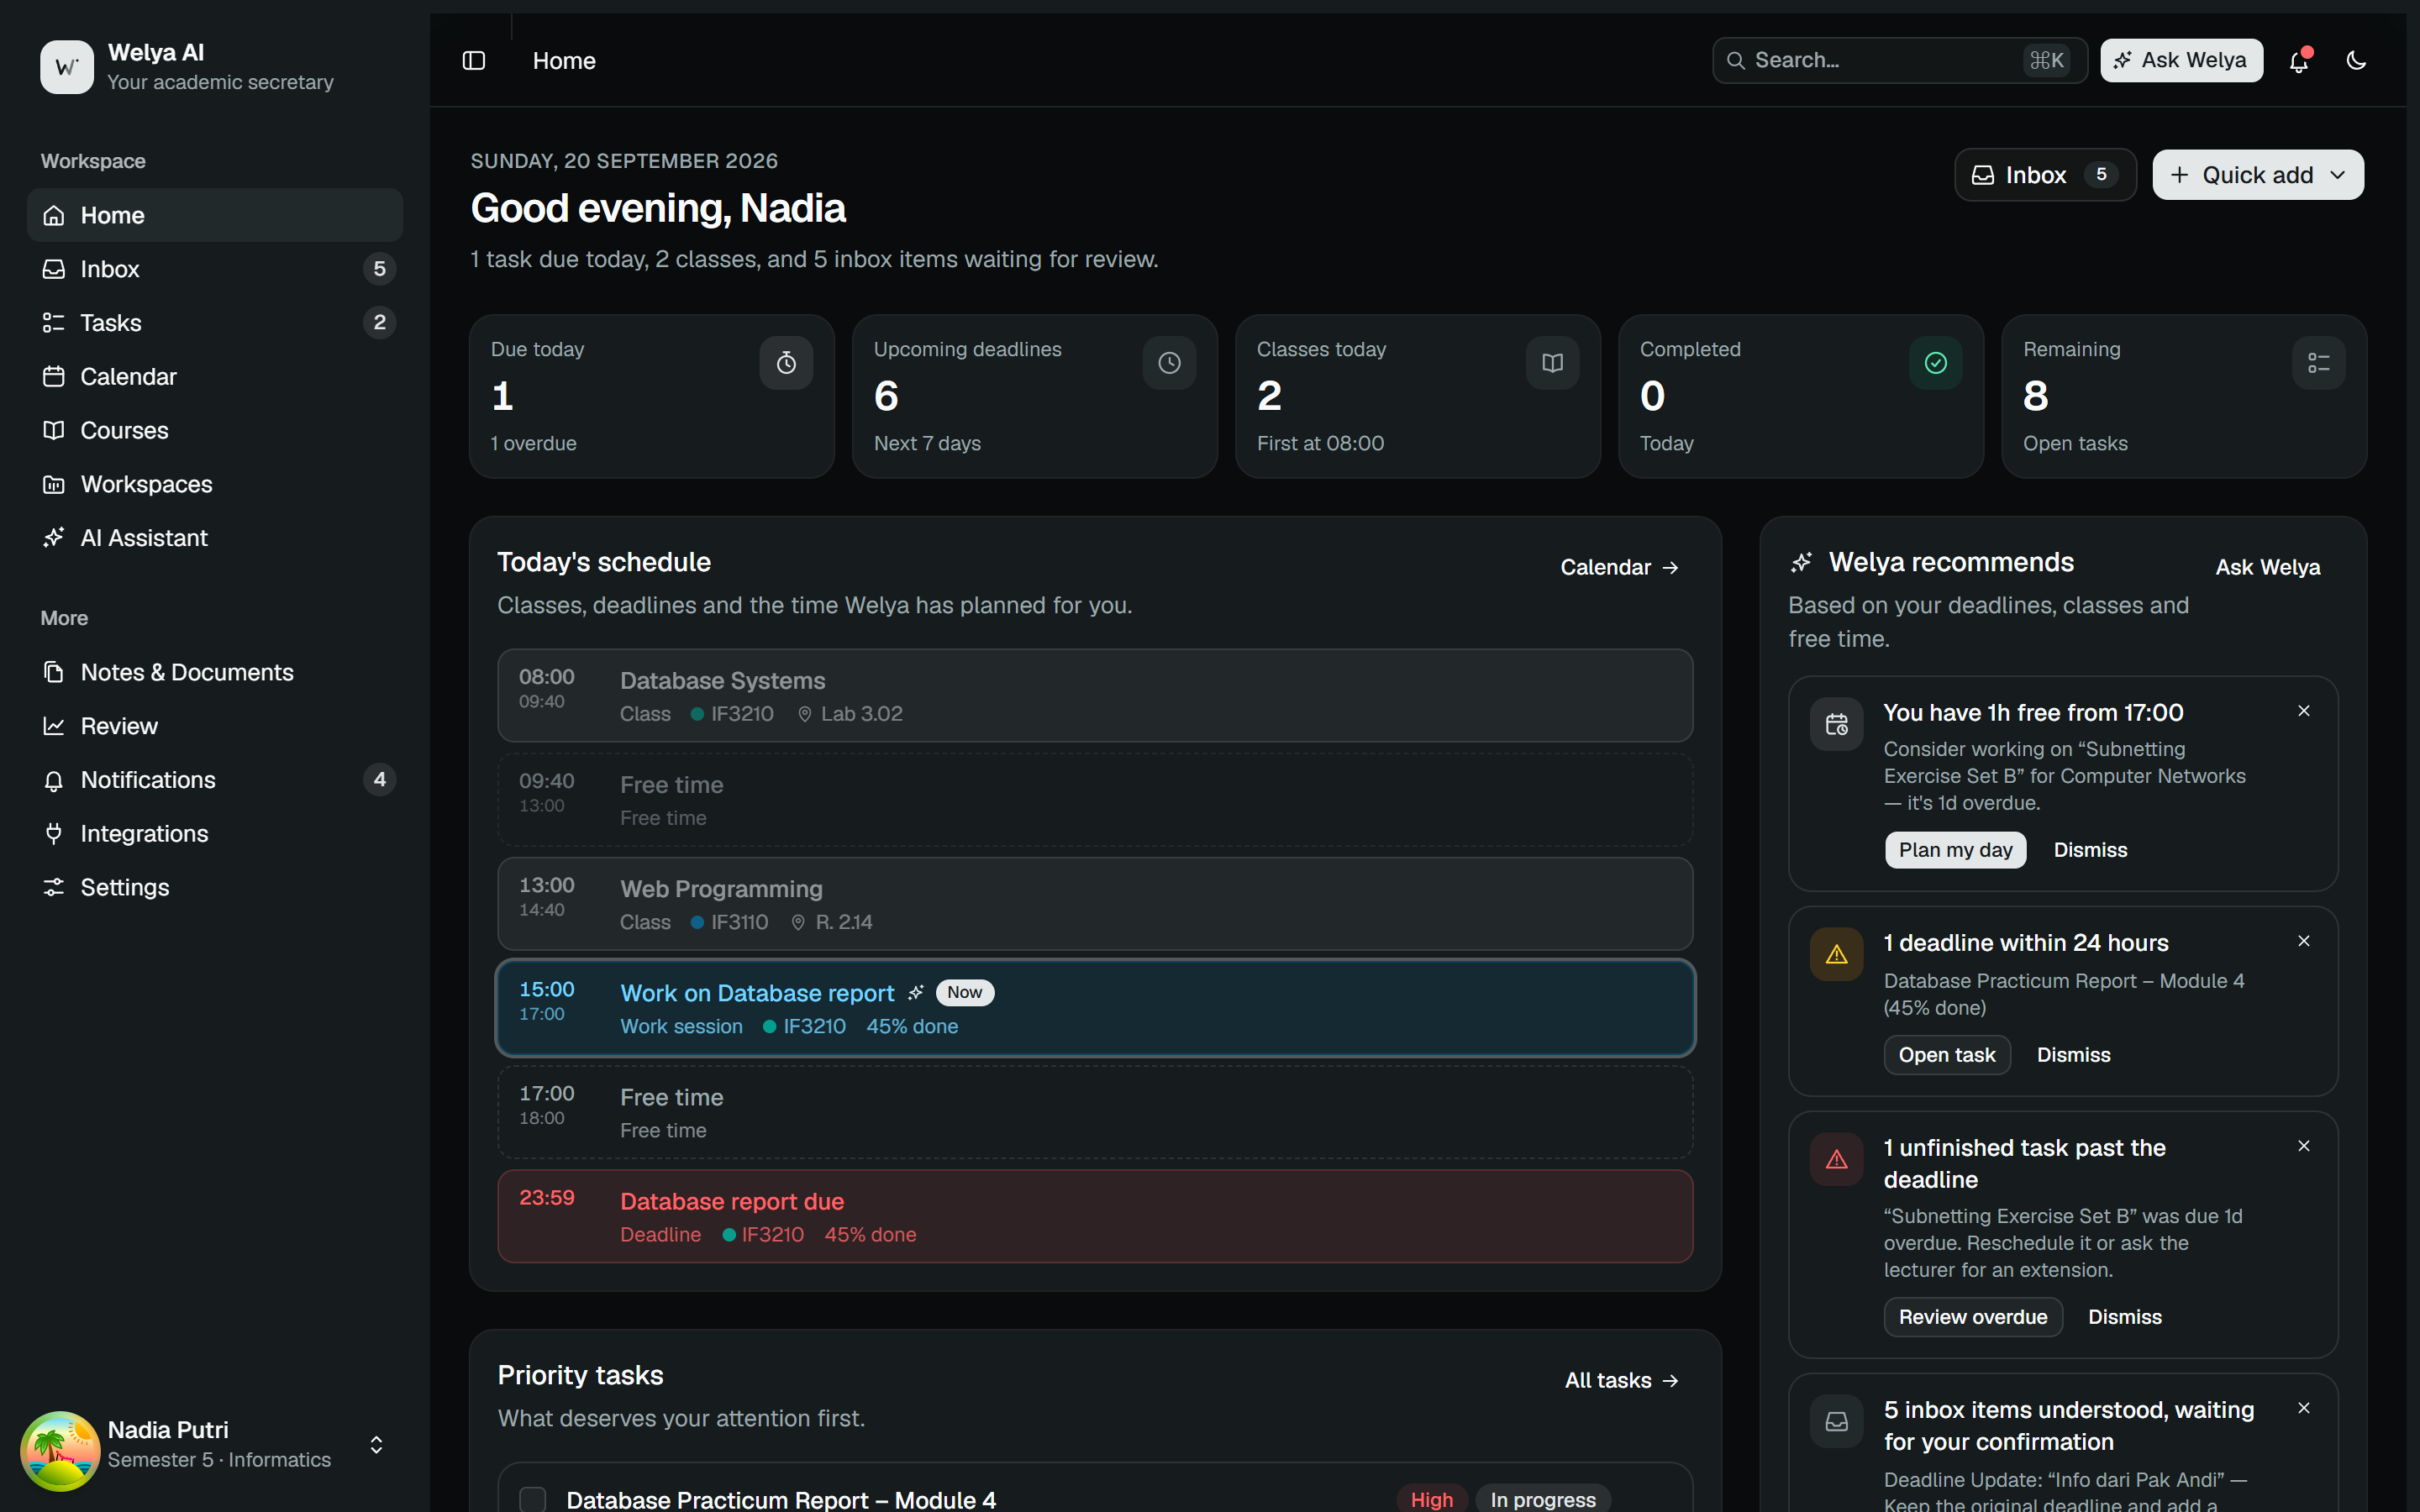
\includegraphics[width=\textwidth]{dashboard-dark}
  \caption{Tampilan dasbor Welya: jadwal hari ini, tugas prioritas beserta
    progres dan subtask, serta rekomendasi dari AI berdasarkan waktu
  luang pengguna}
  \label{gbr:dasbor}
\end{figure}

\begin{figure}[htbp]
  \centering
  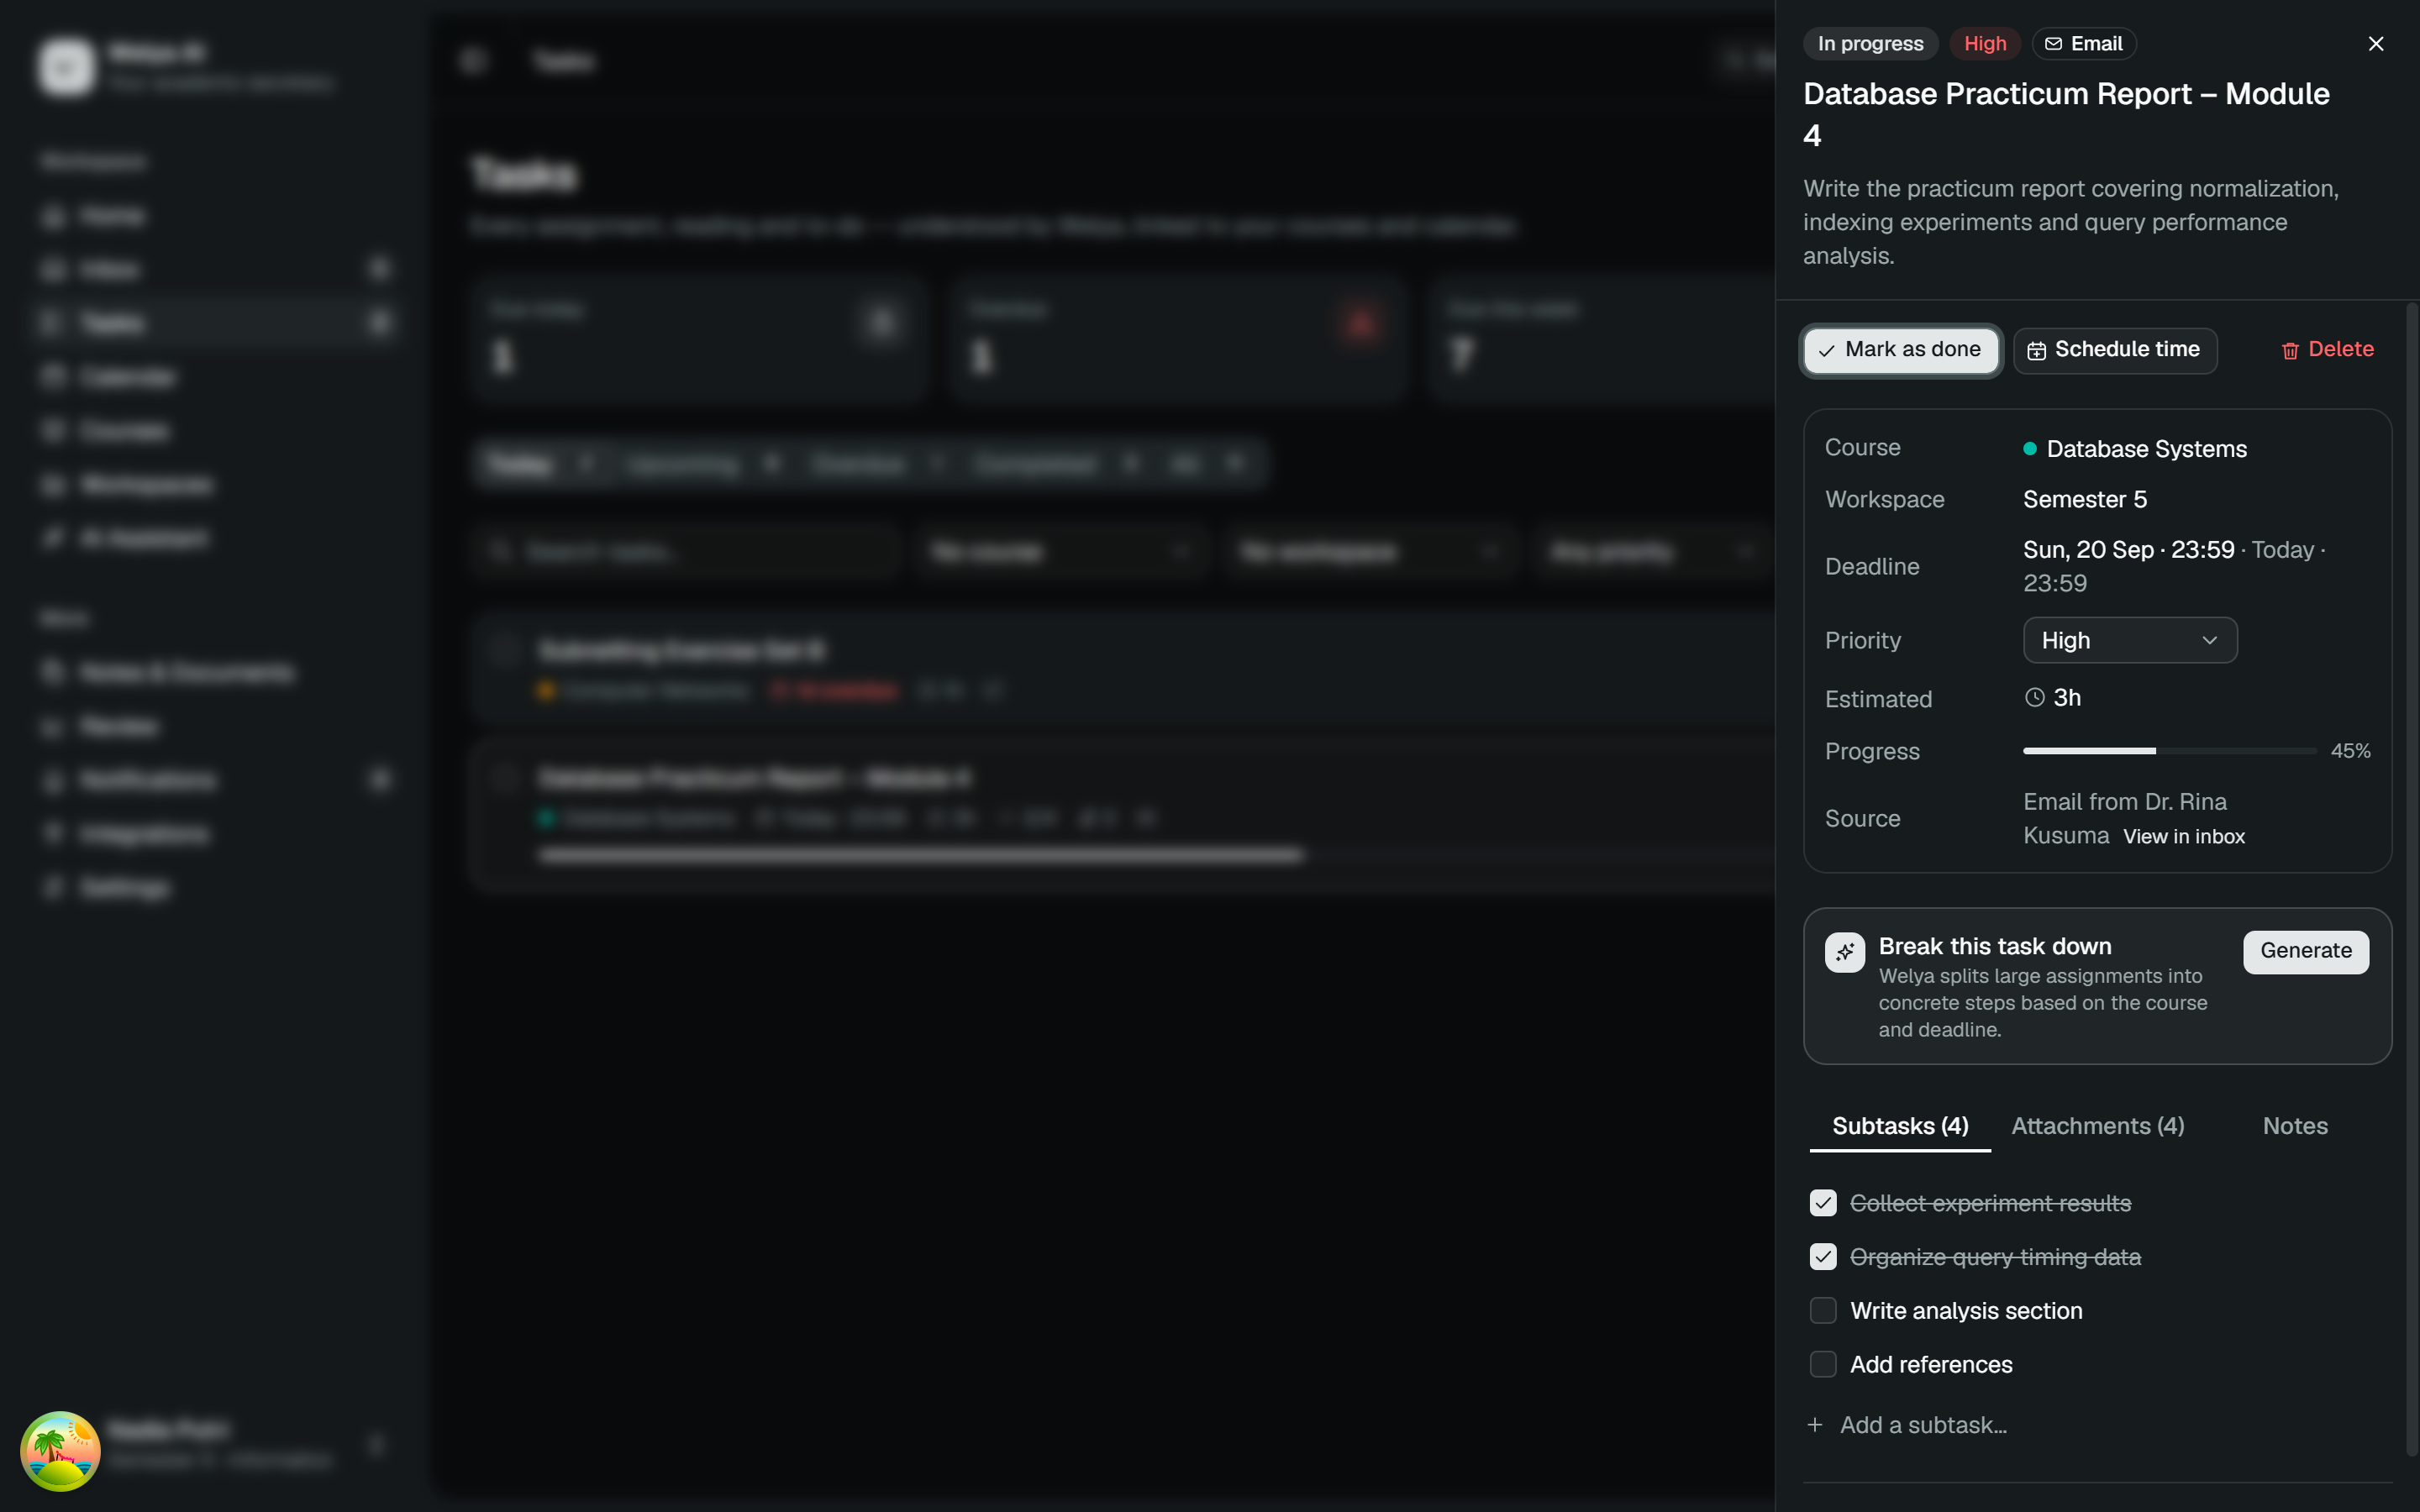
\includegraphics[width=\textwidth]{tasks-dark}
  \caption{Tampilan papan tugas (Tugas Saya) dengan status, prioritas,
  subtask, dan tenggat setiap tugas}
  \label{gbr:tugas}
\end{figure}

\begin{figure}[htbp]
  \centering
  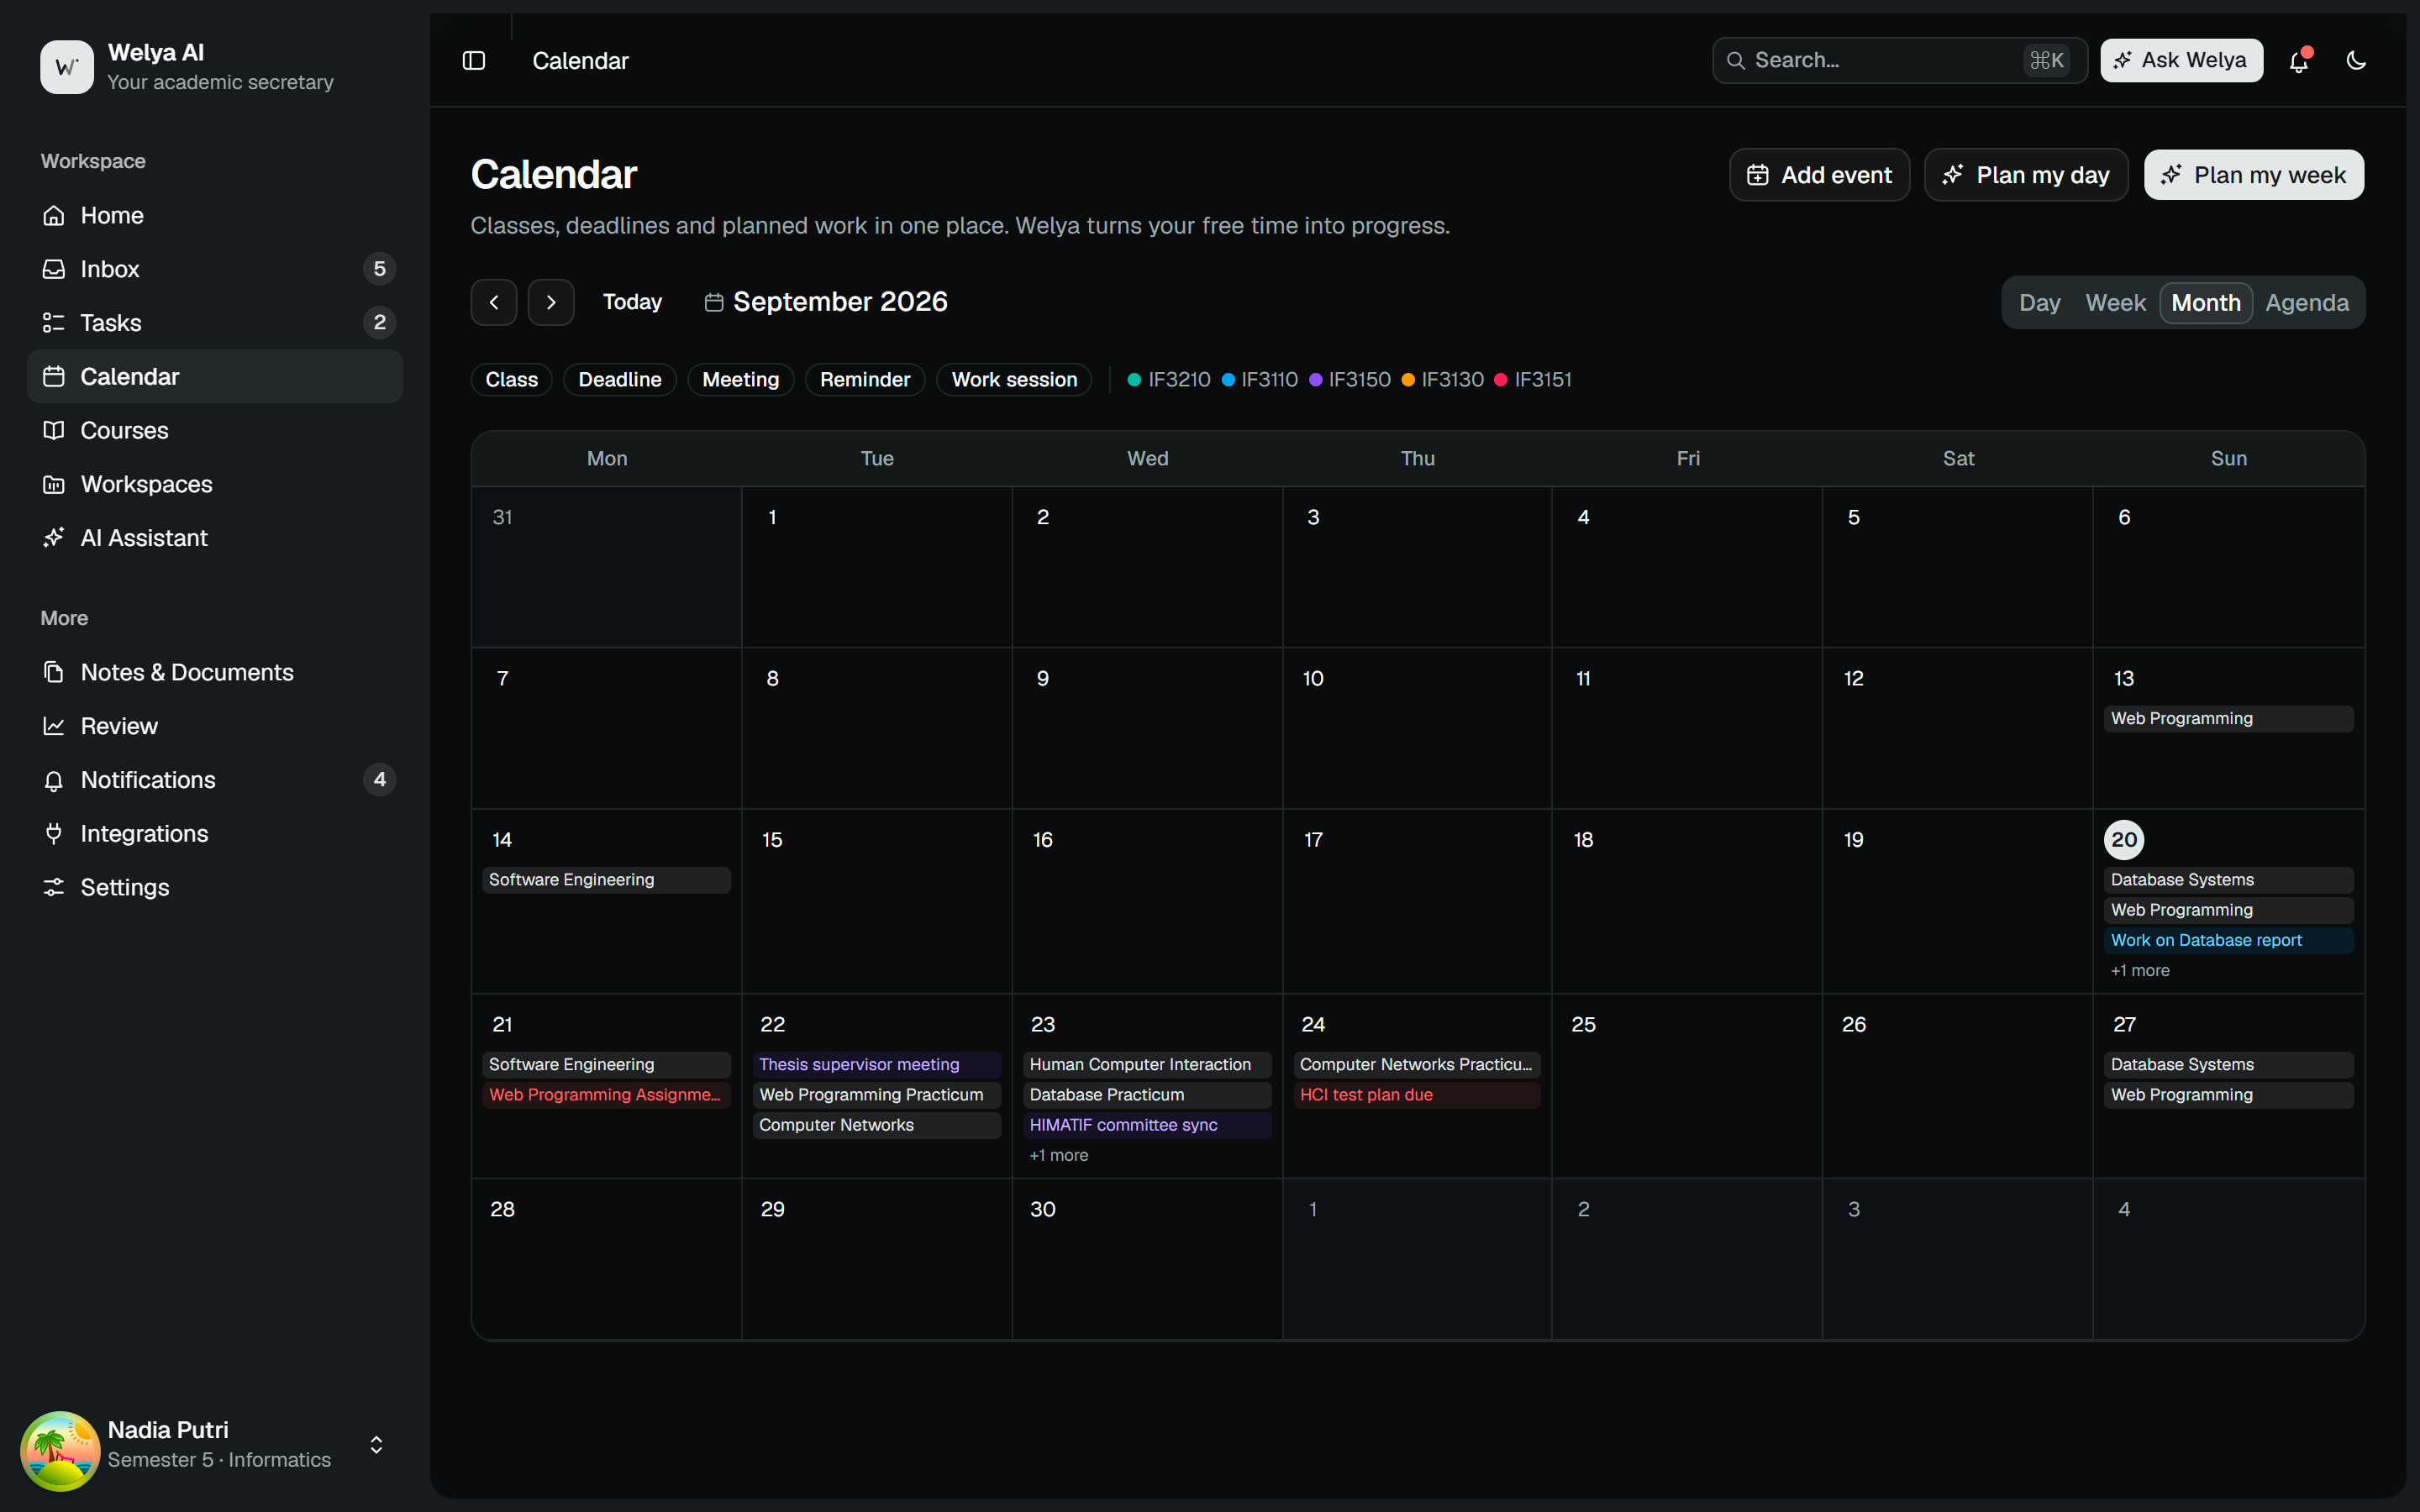
\includegraphics[width=\textwidth]{calendar-dark}
  \caption{Tampilan kalender yang menyatukan jadwal kuliah dan tenggat
  tugas dalam satu tampilan}
  \label{gbr:kalender}
\end{figure}

\begin{figure}[htbp]
  \centering
  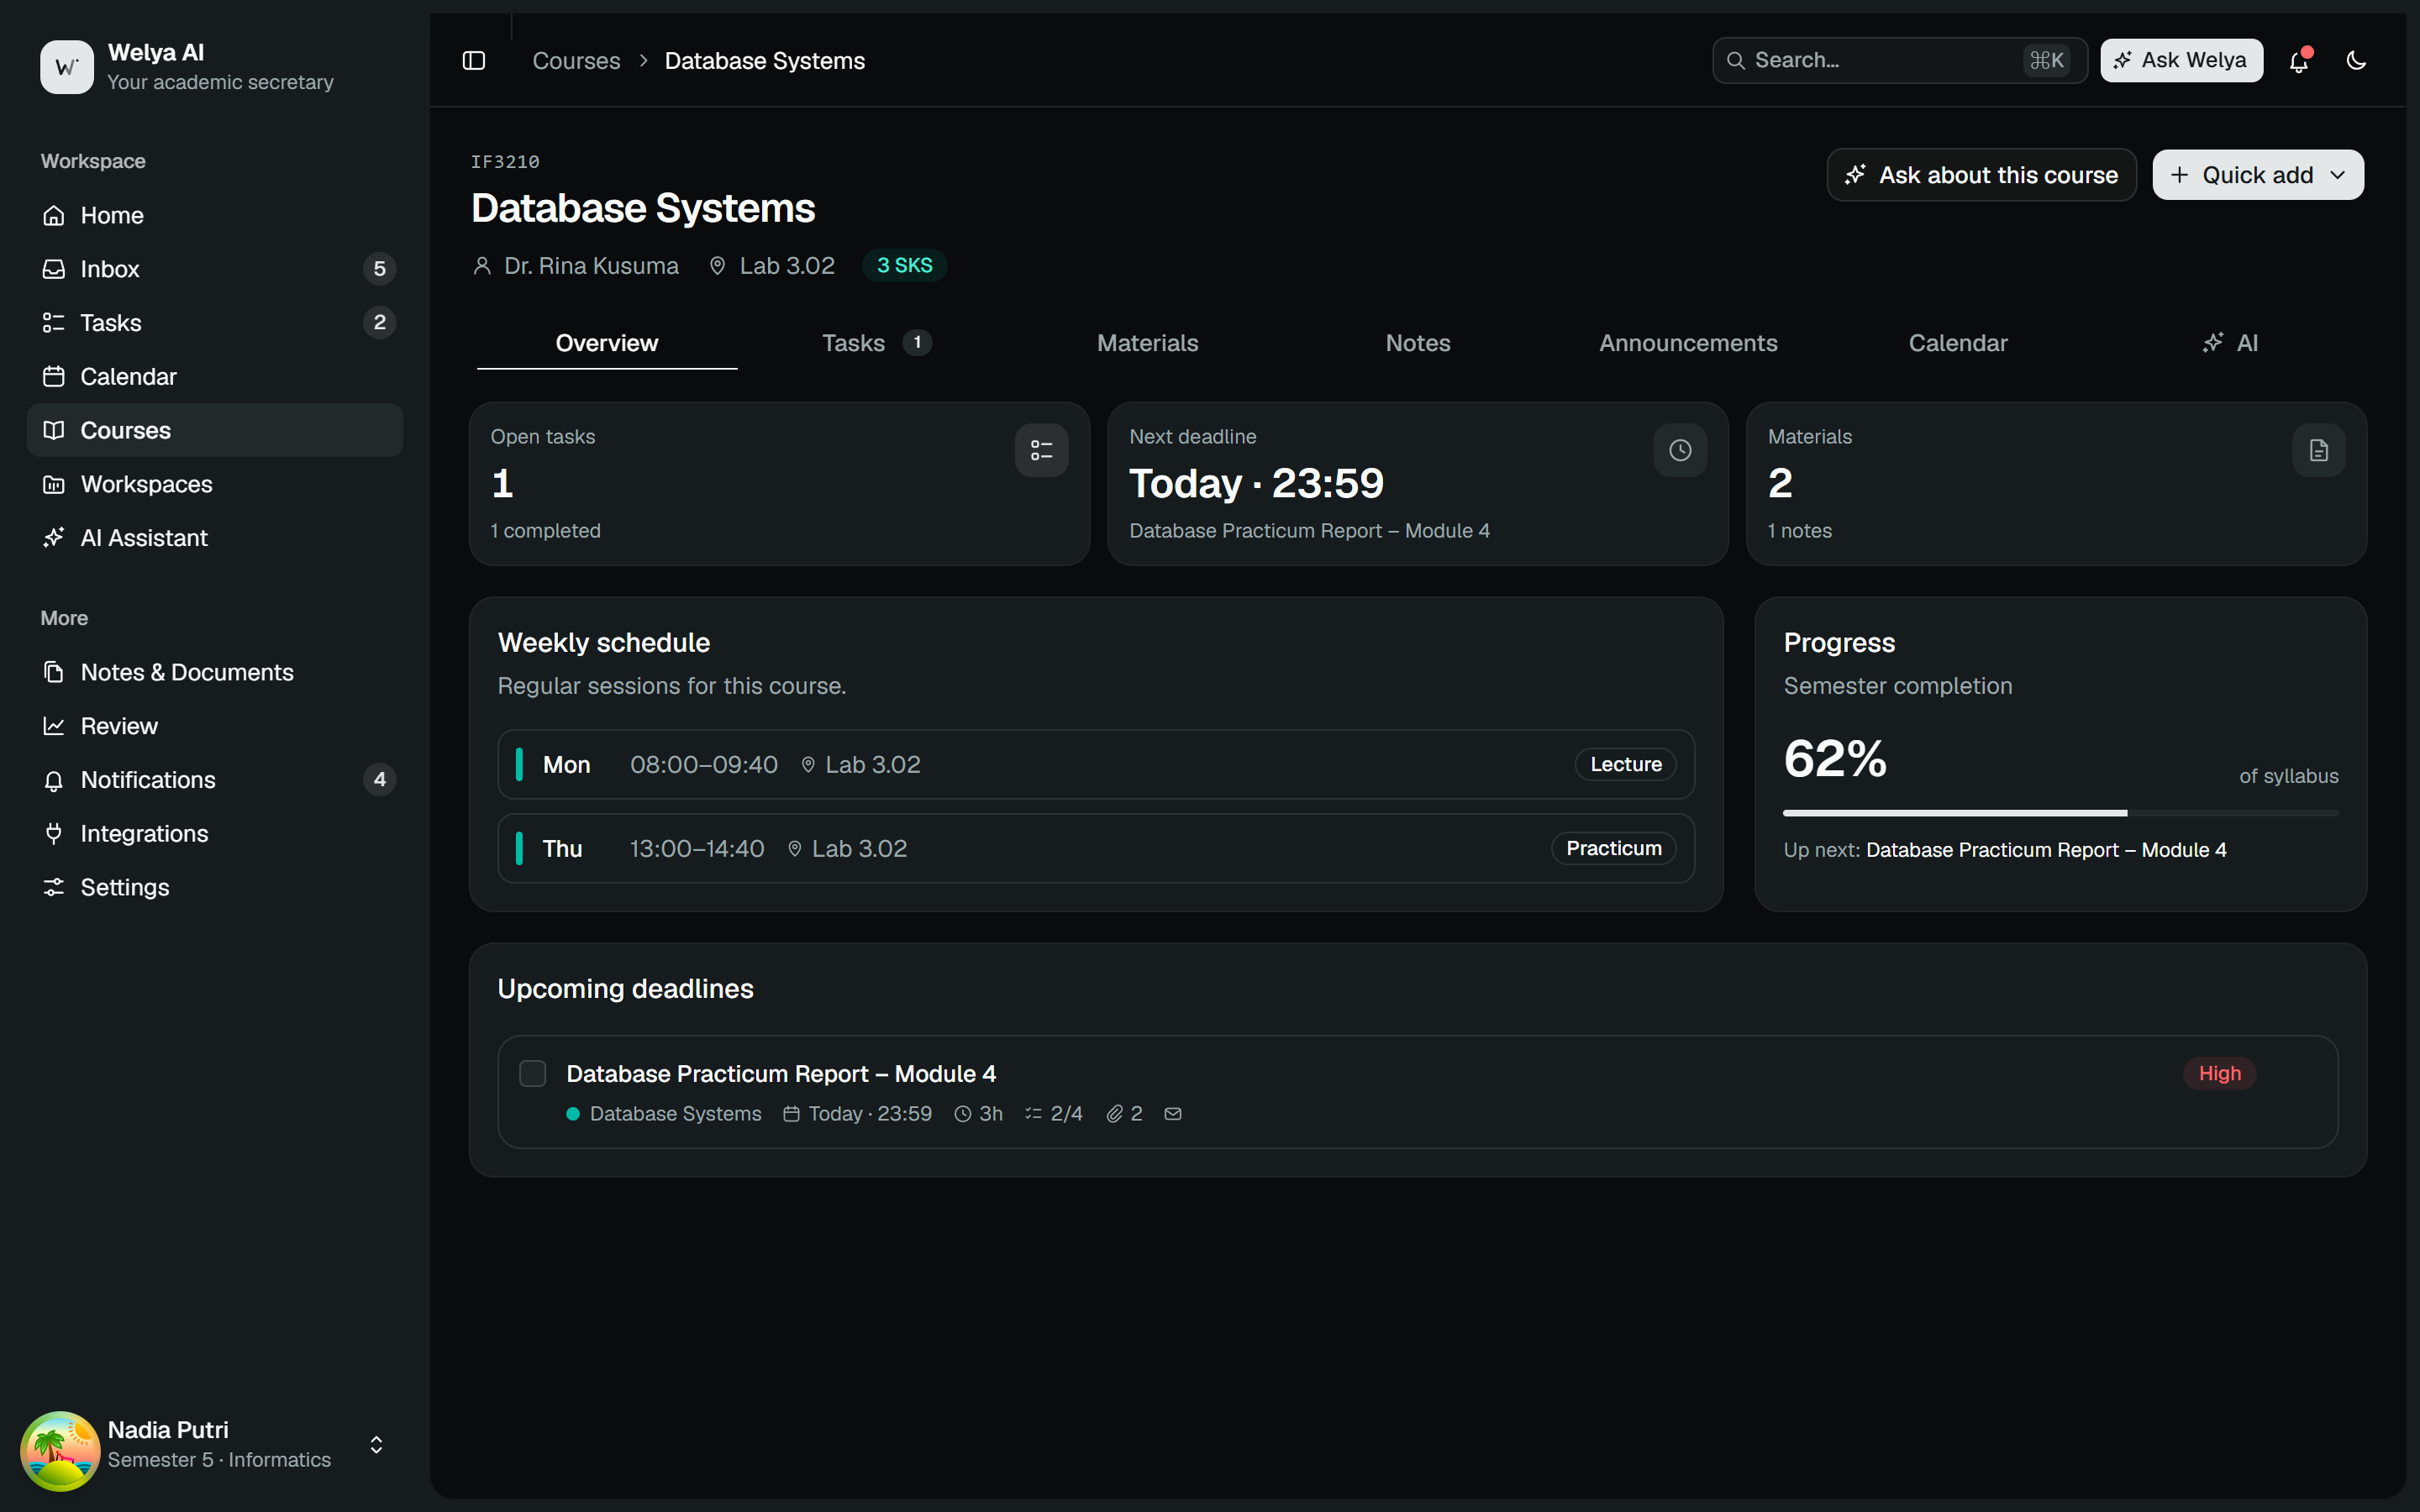
\includegraphics[width=\textwidth]{course-dark}
  \caption{Tampilan ruang mata kuliah: jadwal, tugas, materi, catatan,
  dan pengumuman setiap mata kuliah dalam satu tempat}
  \label{gbr:workspace}
\end{figure}

\clearpage
\section*{Lampiran 2. Perencanaan Teknis}

\subsection*{Rencana Anggaran Biaya (RAB)}
\begin{table}[htbp]
  \centering
  \caption{Rencana anggaran biaya}
  \small
  \begin{tabular}{@{}clrrr@{}}
    \toprule
    No & Uraian & Volume & Harga Satuan (Rp) & Jumlah (Rp) \\
    \midrule
    1 & Domain dan hosting (1 tahun)   & 1 &  &  \\
    2 & Kredit API AI                  & 1 &  &  \\
    3 & Kuota internet pengembangan    & 4 &  &  \\
    4 & Pendaftaran hak cipta (HKI)    & 1 &  &  \\
    5 & Cetak dan jilid laporan        & 3 &  &  \\
    \midrule
    \multicolumn{4}{r}{Total} &  \\
    \bottomrule
  \end{tabular}
\end{table}

\subsection*{Jadwal Kegiatan}
Pengerjaan dilaksanakan pada 3 Agustus--17 September 2026 dengan rincian
pada Tabel~\ref{tab:jadwal}.

\begin{table}[htbp]
  \centering
  \caption{Jadwal kegiatan}
  \label{tab:jadwal}
  \small
  \begin{tabular}{@{}clc@{}}
    \toprule
    No & Kegiatan & Waktu Pelaksanaan \\
    \midrule
    1 & Analisis kebutuhan                   & 3--8 Agustus 2026              \\
    2 & Perancangan sistem                   & 10--15 Agustus 2026            \\
    3 & Implementasi                         & 17 Agustus--5 September 2026   \\
    4 & Pengujian                            & 31 Agustus--11 September 2026  \\
    5 & Evaluasi \& penyusunan laporan       & 7--15 September 2026           \\
    6 & Artikel publikasi \& pendaftaran HKI & 14--17 September 2026          \\
    \bottomrule
  \end{tabular}
\end{table}

\clearpage
\section*{Lampiran 3. Dokumen Pendukung Mitra (khusus TTG)}
Surat pernyataan kerja sama, profil mitra, dan bukti kebutuhan mitra
(kondisi lapangan) dilampirkan di sini apabila tugas akhir dikategorikan
sebagai TTG dengan mitra.


\end{document}
